\documentclass{article}

\usepackage[square,numbers]{natbib}
\usepackage[colorlinks=true, citecolor=black]{hyperref}
\bibliographystyle{unsrtnat}

\usepackage[utf8]{inputenc}
\usepackage[margin=2cm]{geometry}
\usepackage{graphicx}
\usepackage{multirow}
\usepackage{amssymb}
\usepackage{amsmath}
\usepackage{setspace}
\usepackage{outlines}
\usepackage{enumitem}
\usepackage{xcolor}
\usepackage{upgreek}
\usepackage{mathabx}
\usepackage{algorithm}
\usepackage{algorithmic}
\usepackage{amsthm}
\usepackage[labelfont=bf,font=small]{caption}
\usepackage{epsfig}
\usepackage{geometry}
\usepackage{subfigure}
\usepackage[textsize=tiny]{todonotes}
\usepackage[normalem]{ulem}
\usepackage{lipsum}
\usepackage{array}
\usepackage{booktabs}
\usepackage{lineno}
\usepackage{array}
\usepackage{tikz}
\usepackage[english]{babel}
\usepackage{animate}
\usepackage{cancel}

\usepackage[]{siunitx}
\sisetup{range-units=single,separate-uncertainty = true,print-unity-mantissa=false,per-mode=symbol,range-phrase = \text{--},
inter-unit-product=\cdot
}

\usepackage[
    protrusion=true,
    activate={true,nocompatibility},
    final,
    tracking=true,
    kerning=true,
    spacing=true,
    factor=1100]{microtype}
    
\SetTracking{encoding={*}, shape=sc}{40}

\usepackage{outlines}
\usepackage{enumitem}

\definecolor{lightblue}{rgb}{0.63, 0.74, 0.78}
\definecolor{seagreen}{rgb}{0.18, 0.42, 0.41}
\definecolor{orange}{rgb}{0.85, 0.55, 0.13}
\definecolor{silver}{rgb}{0.69, 0.67, 0.66}
\definecolor{rust}{rgb}{0.72, 0.26, 0.06}
\definecolor{purp}{RGB}{68, 14, 156}

\definecolor{zblue}{RGB}{8,81,156}
\definecolor{zpurp}{RGB}{84,39,143}
\definecolor{zred}{RGB}{165,15,21}

\colorlet{lightrust}{rust!50!white}
\colorlet{lightorange}{orange!25!white}
\colorlet{lightlightblue}{lightblue}
\colorlet{lightsilver}{silver!30!white}
\colorlet{darkorange}{orange!75!black}
\colorlet{darksilver}{silver!65!black}
\colorlet{darklightblue}{lightblue!65!black}
\colorlet{darkrust}{rust!85!black}
\colorlet{darkseagreen}{seagreen!85!black}



\usepackage{hyperref}
\hypersetup{
  colorlinks=true,
}
\usepackage{tabularx}
\usepackage{bbm}
\usepackage{bm}

\usepackage[nameinlink]{cleveref}
\crefname{equation}{}{}
\def\appendixname{}
\crefname{appendix}{}{}


\usepackage{setspace}
% \doublespacing
\setlength{\heavyrulewidth}{1.5pt}
% \setlength{\abovetopsep}{4pt}
 
\usepackage{soul}
\sethlcolor{yellow}

\usepackage[parfill]{parskip}

\usepackage{lineno}
\usepackage{tcolorbox}
%\linenumbers

%% Self-defined Macros
\newcommand{\bn}[1]{\mathbf{#1}}
\newcommand{\bs}[1]{\ensuremath{\boldsymbol{#1}}}
\newcommand{\mc}[1]{\ensuremath{\mathcal{#1}}}
\newcommand{\norm}[1]{\ensuremath \lVert #1 \rVert}
\newcommand{\GD}[1]{ D #1 (\boldsymbol{F})[\boldsymbol{H}]}
\newcommand{\GDI}[1]{ D #1 (\boldsymbol{I})[\boldsymbol{H}]}
\newcommand{\Lin}[1]{ L_{\boldsymbol{F}} #1 [\boldsymbol{H}]}
\newcommand{\LinI}[1]{ L_{\boldsymbol{I}} #1 [\boldsymbol{H}]}
\newcommand{\Dm}[1]{\ensuremath{\boldsymbol{\varphi} } }
\newcommand{\tr}[1]{\textcolor{red}{#1}}
\newcommand{\ignore}[1]{}
\newcommand{\fracp}[2]{\frac{\partial #1}{\partial #2}}
\newcommand{\wt}[1]{\widetilde{#1}}
\renewcommand{\[}{\left[}
\renewcommand{\]}{\right]}
\renewcommand{\(}{\left(}
\renewcommand{\)}{\right)}
\newcommand{\tn}{\textnormal}
\newcommand{\gradX}{\nabla_{\bm{X}}}
\newcommand{\gradx}{\nabla_{\bm{x}}}
\newcommand{\gradF}{\nabla_{\bn{F}}}

%\newcommant{\pfrac[2]}{\frac{\partial {#1}}{\partial {#2}}}

%% Coloring for comments
\usepackage{color,tikz,soul}
\newcommand{\jbe}[1]{\textcolor{violet}{#1}}

\newcommand{\rev}[1]{\textcolor{red}{#1}}

\usepackage{xcolor, soul}
\sethlcolor{yellow}
\usepackage[per-mode=symbol]{siunitx}

\setlength{\tabcolsep}{12pt}

\renewcommand{\thetable}{\arabic{table}} % Originally Roman uppercase


\title{MECHENG 517---Mechanics of Soft Materials}
\author{Hyun Jun Ha}
\date {Fall 2025}

\setlength{\marginparwidth}{2cm}

\begin{document}

\maketitle

\section*{Project I: Topic ID and Overview}

I first came across the field of soft tissue mechanics when I received an email about a summer research opportunity in Prof. Arruda's lab. At that time, most of my experiences revolved around my interest in the automotive industry, so I didn't meet many of the listed qualifications. But, because I had yet to find something to do for the summer, I decided to apply anyway. It was the first research opportunity I ever got accepted to, and I was so grateful that I decided to say yes, even though I wasn't very interested in the field. Turns out, it was one of the best decisions I ever made. I enjoyed the balance of both experimental and theoretical work, as well as the need to draw on knowledge from many different areas like mechanics, materials science, and biology. I quickly learned that there are countless unrealized applications in medicine and not many experts in the field. I was motivated by the fact that my work could help someone feel less pain one day, and that if I don't do it, there aren't enough people in the world who would or could.

From my experience, the field of soft tissue mechanics can be divided into three main areas: measurement, modeling, and application. Measurement refers to studying the structure and properties of soft tissues in real life through methods such as magnetic resonance imaging (MRI) or digital image correlation (DIC). Modeling refers to simulating and predicting the behavior of soft tissues, which could involve calculating constitutive parameters or developing finite element models. Lastly, application refers to using those measurements and models to improve patient outcomes in healthcare. Most soft tissues like tendons are composite materials, made up of collagen fibers embedded in an extracellular matrix. They can undergo very large strains and exhibit highly non-linear behaviors that can be described using both visco- and hyperelastic models, which are the main topics of this course. They also accumulate damage and can fail over time, something we'll learn how to model later in the semester. Thus, this course will allow me to explore different ways of modeling the mechanical behavior of soft tissues, as well as some experimental techniques for doing so. I plan to use this knowledge to evaluate and improve existing surgical methods for repairing damaged tissues.

As the global population continues to age, soft tissue injuries such as tendon tears are becoming more common, but many surgical repairs have high failure rates. Most clinical studies on this issue are based on observations rather than mechanistic explanations, and biomechanics studies tend to focus more on forces and stresses instead of deformations and strains. With a better understanding of soft tissue mechanics, physicians could make more informed decisions on when and how to surgically repair injured tissues. For example, they could run an MRI test on a patient's rotator cuff and input the results into a program to predict the chances of a full tear. The repair technique could be optimized to the unique structure and properties of the patient's tissue, as well as the severity of the injury, which could significantly improve surgical outcomes. Thus, advancing the knowledge of soft tissue mechanics could help restore the independence of older adults, improve their quality of life, and reduce the economic costs associated with tissue injuries.

\newpage


\section*{Examples I. Mathematical Preliminaries}

\subsection*{1--1. \textbf{Convolutional integrals} [4 pts].}

(a) 

\begin{equation*}
    \sigma_1(\tau) = \sigma_0 H(\tau)
\end{equation*}

\begin{equation*}
    \frac{d\sigma_1(\tau)}{d\tau} = \sigma_0\delta(\tau)
\end{equation*}

\begin{equation}
    \varepsilon_1(t) = \sigma_0 \int_0^t J(t-\tau) \delta(\tau) d\tau,
\end{equation}

where $\delta(\tau)$ is the signal and $J(t-\tau)$ is the filter function.

\bigskip

\begin{equation*}
    \mathcal{L}\{\delta(t)\} =1
\end{equation*}

\begin{equation*}
     \mathcal{L}\{J(t)\} = \mathcal{L}\{J_\infty\} + \mathcal{L}\{(J_0-J_\infty)e^{-t/\tau_c}\}
\end{equation*}

\begin{equation*}
    \mathcal{L}\{J(t)\} = \mathcal{L}\{J_\infty\} + (J_0-J_\infty)\mathcal{L}\{e^{-(1/\tau_c)t}\}
\end{equation*}

\begin{equation*}
    \mathcal{L}\{J(t)\} = \frac{J_\infty}{s} + \frac{J_0-J_\infty}{s+1/\tau_c}
\end{equation*}

\bigskip

Since (1) is a convolution integral,

\begin{equation*}
    \mathcal{L}\{\varepsilon_1(t)\} = \sigma_0*\mathcal{L}\{\delta(t)\}*\mathcal{L}\{J(t)\}
\end{equation*}

\begin{equation*}
    \mathcal{L}\{\varepsilon_1(t)\} = \sigma_0*1*(\frac{J_\infty}{s} + \frac{J_0-J_\infty}{s+1/\tau_c})
\end{equation*}

\begin{equation*}
    \mathcal{L}\{\varepsilon_1(t)\} = \frac{J_\infty\sigma_0}{s} + \frac{(J_0-J_\infty)\tau_c\sigma_0}{\tau_cs+1}
\end{equation*}

\newpage


(b)

\begin{equation*}
    \sigma_2(\tau) = \sigma_0 sin(\omega \tau)
\end{equation*}

\begin{equation*}
    \frac{d\sigma_2(\tau)}{d\tau} = \sigma_0 \omega cos(\omega \tau)
\end{equation*}

\begin{equation}
    \varepsilon_2(t) = \sigma_0 \omega \int_0^t J(t-\tau) cos(\omega \tau) d\tau,
\end{equation}

where $cos(\omega \tau)$ is the signal and $J(t-\tau)$ is the filter function.

\bigskip

\begin{equation*}
    \mathcal{L}\{\cos(\omega t)\} = \frac{s}{s^2+\omega^2}
\end{equation*}

\begin{equation*}
    \mathcal{L}\{J(t)\} = \frac{J_\infty}{s} + \frac{J_0-J_\infty}{s+1/\tau_c}
\end{equation*}

\bigskip

Since (2) is a convolution integral,

\begin{equation*}
    \mathcal{L}\{\varepsilon_2(t)\} = \sigma_0\omega*\mathcal{L}\{cos(\omega\tau)\}*\mathcal{L}\{J(t)\}
\end{equation*}

\begin{equation*}
    \mathcal{L}\{\varepsilon_2(t)\} = \sigma_0\omega*\frac{s}{s^2+\omega^2}*(\frac{J_\infty}{s} + \frac{J_0-J_\infty}{s+1/\tau_c})
\end{equation*}

\begin{equation*}
    \mathcal{L}\{\varepsilon_2(t)\} = \frac{J_\infty\sigma_0\omega}{s^2+\omega^2} + \frac{(J_0-J_\infty)(\tau_c\sigma_0\omega)s}{\tau_c s^3+s^2+\tau_c\omega^2 s+\omega^2}
\end{equation*}

\newpage


\subsection*{1--2. \textbf{Index notation} [4 pts].}

Let $\bm{w}=\bm{q} \times \bm{r}$,

\begin{equation*}
    \bm{p} \times \bm{w} = \epsilon_{ijk} p_j w_k
\end{equation*}

\begin{equation*}
    = \epsilon_{ijk} p_j (\epsilon_{klm} q_l r_m)
\end{equation*}

\begin{equation*}
    = (\epsilon_{kij} \epsilon_{klm}) p_j q_l r_m
\end{equation*}

\begin{equation*}
    = (\delta_{il} \delta_{jm} - \delta_{im} \delta_{jl}) p_j q_l r_m
\end{equation*}

\begin{equation*}
    = p_j q_l r_m \delta_{il} \delta_{jm} - p_j q_l r_m \delta_{im} \delta_{jl}
\end{equation*}

\begin{equation*}
    = (p_j r_m \delta_{jm}) q_l \delta_{il} - (p_j q_l \delta_{jl}) r_m \delta_{im}
\end{equation*}

\begin{equation*}
    = (r_j p_j) q_i - (q_j p_j) r_i
\end{equation*}

\begin{equation*}
    = (\bm{r} \cdot \bm{p}) \bm{q} - (\bm{q} \cdot \bm{p}) \bm{r}
\end{equation*}

\newpage


Let $\bm{u} = \bm{p} \times \bm{q}$ and $\bm{v} = \bm{a} \times \bm{b}$

\begin{equation*}
    \bm{u} \cdot \bm{v} = u_i v_i
\end{equation*}

\begin{equation*}
    = (\epsilon_{ikl} p_k q_l) (\epsilon_{imn} a_m b_n)
\end{equation*}

\begin{equation*}
    = (\delta_{km} \delta_{ln} - \delta_{kn} \delta_{lm}) p_k q_l a_m b_n
\end{equation*}

\begin{equation*}
    = \delta_{km} \delta_{ln} p_k q_l a_m b_n - \delta_{kn} \delta_{lm} p_k q_l a_m b_n
\end{equation*}

\begin{equation*}
    = (p_k a_m \delta_{km}) (q_l b_n \delta_{ln}) - (p_k b_n \delta_{kn}) (q_l a_m \delta_{lm})
\end{equation*}

\begin{equation*}
    = (p_k a_k)(q_l b_l) - (q_l a_l)(p_k b_k)
\end{equation*}

\begin{equation*}
    = (\bm{p} \cdot \bm{a}) (\bm{q} \cdot \bm{b}) - (\bm{q} \cdot \bm{a})(\bm{p} \cdot \bm{b})
\end{equation*}

\newpage


\begin{equation*}
    (\bm{a} \otimes \bm{b})(\bm{p} \otimes \bm{q}) = (a_i b_j(\bm{e}^{(i)} \otimes \bm{e}^{(j)})(p_k q_l(\bm{e}^{(k)} \otimes \bm{e}^{(l)})
\end{equation*}

\begin{equation*}
    = 
\end{equation*}


\begin{equation*}
    = \bm{a}\otimes\bm{q}(\bm{b} \cdot \bm{p})
\end{equation*}

\newpage


\begin{equation*}
    \bm{Q}^\intercal \bm{a} \cdot \bm{Q}^\intercal \bm{b} = 
\end{equation*}


\begin{equation*}
    = \bm{a} \cdot \bm{b}
\end{equation*}

\newpage


\subsection*{1--4. \textbf{Vector and tensor calculus} [4 pts].} Show the following vector and tensor identities to be true using index notation:

\begin{equation*}
    \gradX \times (\phi \bm{a}) = \epsilon_{ijk} (\phi a)_{k,j} \bm{e}_{i}
\end{equation*}

\begin{equation*}
    = \epsilon_{ijk}(a_k \phi_{,j} + \phi a_{k,j})\bm{e}_{i}
\end{equation*}

\begin{equation*}
    = \epsilon_{ijk} a_k \phi_{,j} \bm{e}_{i} + \epsilon_{ijk} \phi a_{k,j} \bm{e}_{i}
\end{equation*}

\begin{equation*}
    = \phi(\epsilon_{ijk}  a_{k,j} \bm{e}_{i}) + \epsilon_{ijk} \phi_{,j} a_k \bm{e}_{i}
\end{equation*}

\begin{equation*}
    = \phi \gradX \times \bm{a} + (\gradX\phi) \times \bm{a}
\end{equation*}

\newpage


\begin{equation*}
    \gradX (\bm{a} \cdot \bm{b}) = (a_j b_j)_i \bm{e}_i
\end{equation*}

\begin{equation*}
    = (b_j a_{j,i} + a_j b_{j,i}) \bm{e}_i
\end{equation*}

\bigskip

\begin{equation*}
    (\bm{a} \cdot \gradX) \bm{b} = a_j b_{i,j}
\end{equation*}

\begin{equation*}
    (\bm{b} \cdot \gradX) \bm{a} = b_j a_{i,j}
\end{equation*}

\begin{equation*}
    \bm{a} \times (\gradX \times \bm{b}) = \epsilon_{ijk} a_j (\epsilon_{klm} b_{m,l} \bm{e}_k)
\end{equation*}

\begin{equation*}
    = (\epsilon_{kij} \epsilon_{klm}) a_j b_{m,l} \bm{e}_k
\end{equation*}

\begin{equation*}
    = (\delta_{il} \delta_{jm} - \delta_{im} \delta_{jl}) a_j b_{m,l} \bm{e}_k
\end{equation*}

\begin{equation*}
    = \delta_{il} \delta_{jm} a_j b_{m,l} \bm{e}_k - \delta_{im} \delta_{jl} a_j b_{m,l} \bm{e}_k
\end{equation*}

\begin{equation*}
    \bm{b} \times (\gradX \times \bm{a}) = \epsilon_{ijk} b_j (\epsilon_{klm} a_{m,l} \bm{e}_k)
\end{equation*}

\begin{equation*}
    = (\epsilon_{kij} \epsilon_{klm}) b_j a_{m,l} \bm{e}_k
\end{equation*}

\begin{equation*}
    = (\delta_{il} \delta_{jm} - \delta_{im} \delta_{jl}) b_j a_{m,l} \bm{e}_k
\end{equation*}

\begin{equation*}
    = \delta_{il} \delta_{jm} b_j a_{m,l} \bm{e}_k - \delta_{im} \delta_{jl} b_j a_{m,l} \bm{e}_k
\end{equation*}




\begin{equation*}
    = (\bm{a} \cdot \gradX) \bm{b} + (\bm{b} \cdot \gradX) \bm{a} + \bm{a} \times (\gradX \times \bm{b}) + \bm{b} \times (\gradX \times \bm{a})
\end{equation*}

I ran out of time to solve all the problems, but I'm planning to keep working on them and resubmit the assignment later. Thank you!

\newpage


\section*{Project II: Literature Review}

\begin{outline}
    \1 \textbf{Introductory context}
        \2 Synthetic, polymer patches were first used in the 1980s to repair massive rotator cuff tears \cite{ozaki1986reconstruction}, but with increasing prevalence \cite{yamaguchi2006demographic} and persistently high re-tear rates of 20\% \cite{longo2021retear}, current research has focused on using patches to augment suture repairs for all tear sizes \cite{cobb2022rotator}. Patch augmentation provides support to the torn tendon by sharing load with the sutures \cite{shea2012biomechanical} and can significantly reduce re-tear rates \cite{de2022benefits}.
    
    \1 \textbf{The state of the field}
        \2 Patches have been developed mainly for biocompatibility, leading to a focus on extracellular matrix (ECM)-based materials that comprise the majority of commerically-available patches \cite{hakimi2013synthetic}. Some of their mechanical properties have been evaluated in-vivo as part of a full repair \cite{barber2008ultimate, mehta2020biomechanical} and in-vitro by themselves \cite{derwin2006commercial, chaudhury2012tensile} with measurements of load-to-failure, gap formation, and elastic moduli.
        
    \1 \textbf{The Big Gap}
        \2 Although it is well-established that the mechanical properties of an implant should closely match that of native tissue to prevent shielding \cite{vunjak2004tissue}, the properties of patches relative to rotator cuff tendons are largely unknown, especially in terms of their hyper- and viscoelastic behavior. Characterization of biological materials remains difficult due to their complex structure, natural variability, and limited measurement techniques.
\end{outline}

\bibliography{Hyun-Jun-Ha-references}


\newpage


\section*{Examples II. Kinetics, Constitutive Laws, and Viscoelasticity I}

\subsection*{2--1. \textbf{Balance of mass} [4 pts].}

\begin{equation*}
    \frac{\partial \rho}{\partial t} + \gradX \cdot (\rho \bm{v}) = 0
\end{equation*}

\begin{equation*}
    \frac{\partial \rho}{\partial t} + \frac{1}{r^2} \frac{\partial (r^2 \rho v_r)}{\partial r} + \frac{1}{r \sin \theta} \frac{\partial (\rho v_\theta \sin \theta)}{\partial \theta} + \frac{1}{r \sin \theta} \frac{\partial \rho v_z}{\partial z} = 0
\end{equation*}

\begin{equation*}
    \frac{\partial \rho}{\partial t} + \frac{1}{r^2} (\rho v_r \frac{\partial r^2}{\partial r}+ r^2v_r \frac{\partial \rho}{\partial r} + r^2 \rho \frac{\partial v_r}{\partial r}) + 0 + 0 = 0
\end{equation*}

\begin{equation*}
    \rho_{,t} + \frac{2 \rho v_r}{r} + v_r \rho_{,r} + \rho v_{r,r} = 0
\end{equation*}

\begin{equation*}
    \rho_{,t} + \rho_{,r} v_r + \frac{\rho}{r}(2v_r + r v_{r,r}) = 0
\end{equation*}

\newpage


\begin{equation*}
    \gradX \cdot \bm{v} = 0
\end{equation*}

\begin{equation*}
    \frac{1}{r^2} \frac{d r^2 v_r}{d r} = 0
\end{equation*}

\begin{equation*}
    \frac{1}{r^2} (v_r \frac{d r^2}{d r} + r^2 \frac{d v_r}{d r}) = 0
\end{equation*}

\begin{equation*}
    \frac{2v_r}{r} + \frac{d v_r}{d r} = 0
\end{equation*}

\begin{equation*}
    \frac{2v_r}{r} = - \frac{d v_r}{d r}
\end{equation*}

\begin{equation*}
    \frac{1}{r}dr = -\frac{1}{2v_r}dv_r
\end{equation*}

\begin{equation*}
    \int_{R}^{r} \frac{1}{r}dr = \int_{\dot R}^{v_r} -\frac{1}{2v_r}dv_r
\end{equation*}

\begin{equation*}
    \int_{R}^{r} \frac{1}{r}dr = -\frac12 \int_{\dot R}^{v_r} \frac{1}{v_r}dv_r
\end{equation*}

\begin{equation*}
    ln|r| - ln|R| = -\frac12 (ln|v_r| - ln|\dot R|)
\end{equation*}

\begin{equation*}
    ln|\frac{r}{R}| = ln(|\frac{v_r}{\dot R}|^{-\frac12})
\end{equation*}

\begin{equation*}
    \frac{r}{R} = (\frac{v_r}{\dot R})^{-\frac12}
\end{equation*}

\begin{equation*}
    \frac{r}{R} = (\frac{v_r}{\dot R})^{-\frac12}
\end{equation*}

\begin{equation*}
    \frac{R^2}{r^2} = \frac{v_r}{\dot R}
\end{equation*}

\begin{equation*}
    v_r(r,t) = \frac{R^2 \dot R}{r^2}
\end{equation*}

\newpage


\subsection*{2--2. \textbf{Balance of momenta} [4 pts].}




\newpage


\subsection*{2--3. \textbf{Viscoelastic data} [4 pts].} 

(a) The material can be described with linear viscoelasticity but only from $\varepsilon = 0$ to about $\varepsilon = 2$, where the isochrones are linear and their slopes scale with time.

\bigskip

(b)

$\sigma=100$ Pa: $\varepsilon(2) = 0.44$, $\varepsilon(5) = 0.53$, $\varepsilon(10) = 0.67$, $\varepsilon(20) = 0.82$, $\varepsilon(40) = 1$

$\sigma=250$ Pa: $\varepsilon(2) = 1.2$, $\varepsilon(5) = 1.45$, $\varepsilon(10) = 1.8$, $\varepsilon(20) = 2.4$, $\varepsilon(40) = 3$

\begin{figure}[ht]
    \centering
    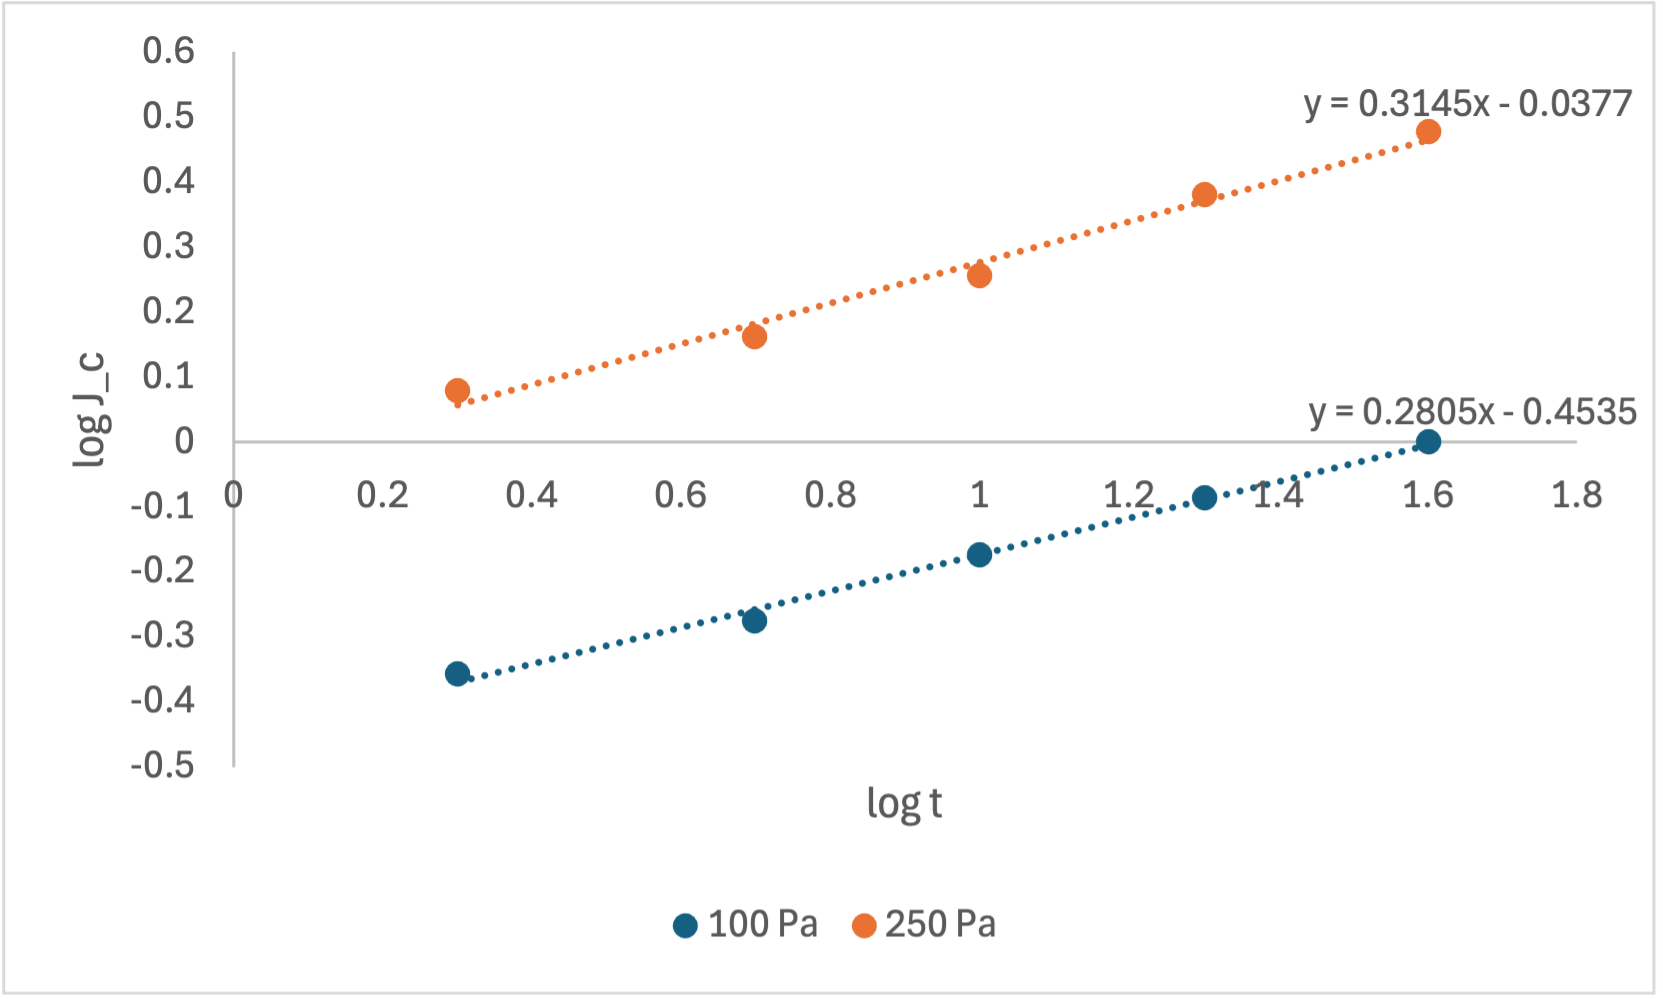
\includegraphics[width=1\linewidth]{Picture1.png}
    \label{fig:placeholder}
\end{figure}

\begin{equation*}
    \log(J_{c,\ 100 Pa}) = 0.2805 \log(t) - 0.4535
\end{equation*}

\begin{equation*}
    J_{c,\ 100 Pa} = 10^{0.2805 \log(t) - 0.4535} = 10^{-0.4535} t^{0.2805} \approx 0.3520 t^{0.2805}
\end{equation*}

\bigskip

\begin{equation*}
    \log(J_{c,\ 250 Pa}) = 0.3145 \log(t) - 0.0377
\end{equation*}

\begin{equation*}
    J_{c,\ 250 Pa} = 10^{0.3145 \log(t) - 0.0377} = 10^{-0.0377} t^{0.3145} \approx 0.9170 t^{0.3145}
\end{equation*}

\newpage


\subsection*{2--4. \textbf{Impulsive stresses} [4 pts].}

(a)

\begin{equation*}
    \varepsilon(t) = \int_{0^-}^{t} J_c(t-\tau) \frac{d\sigma(\tau)}{d\tau} d\tau
\end{equation*}

\begin{equation*}
    \varepsilon(t) = A \int_{0^-}^{t} J_c(t-\tau) \frac{d\delta(\tau)}{d\tau} d\tau
\end{equation*}

\begin{equation*}
    \varepsilon(s) = A \cdot \mathcal{L}(\frac{d\delta(t)}{dt}) \cdot \mathcal{L}(J_c(t)) 
\end{equation*}

\begin{equation*}
    \varepsilon(s) = A \cdot (s \cdot 1 - \delta(0^-)) \cdot J_c(s)
\end{equation*}

\begin{equation*}
    \varepsilon(s) = A \cdot s \cdot J_c(s)
\end{equation*}

\begin{equation*}
    \varepsilon(t) = A \dot J_c(t)
\end{equation*}

\bigskip

\begin{equation*}
    \eta \dot\varepsilon + E \varepsilon(t) = \sigma(t)
\end{equation*}

\begin{equation*}
    \eta \dot\varepsilon + E \varepsilon(t) = A \delta(t)
\end{equation*}

\begin{equation*}
    \dot\varepsilon + \frac{E}{\eta} \varepsilon(t) = \frac{A}{\eta} \delta(t)
\end{equation*}

\begin{equation*}
    \dot\varepsilon e^\frac{Et}{\eta} + \frac{E}{\eta} \varepsilon(t) e^\frac{Et}{\eta} = \frac{A}{\eta} \delta(t) e^\frac{Et}{\eta}
\end{equation*}

\begin{equation*}
    \frac{d}{dt} (\varepsilon(t) e^\frac{Et}{\eta}) = \frac{A}{\eta} \delta(t) e^\frac{Et}{\eta}
\end{equation*}

\begin{equation*}
    \int \frac{d}{dt} (\varepsilon(t) e^\frac{Et}{\eta}) dt = \frac{A}{\eta} \int \delta(t) e^\frac{Et}{\eta} dt
\end{equation*}

\begin{equation*}
    \varepsilon(t) e^\frac{Et}{\eta} = \frac{A}{\eta}
\end{equation*}

\begin{equation*}
    \varepsilon(t) = \frac{A}{\eta} e^{-\frac{Et}{\eta}}
\end{equation*}

\newpage


(b)

\begin{equation*}
    \varepsilon(t) = B \int_{0^-}^{t} J_c(t-\tau) \frac{d\psi(\tau)}{d\tau} d\tau
\end{equation*}

\begin{equation*}
    \varepsilon(s) = B \cdot \mathcal{L}(\frac{d^2\delta(t)}{dt^2}) \cdot \mathcal{L}(J_c(t)) 
\end{equation*}

\begin{equation*}
    \varepsilon(s) = B \cdot (s^2 \cdot 1 - s \cdot \delta(0^-) - \psi(0^-)) \cdot J_c(s)
\end{equation*}

\begin{equation*}
    \varepsilon(s) = B \cdot s^2 \cdot J_c(s)
\end{equation*}

\begin{equation*}
    \varepsilon(t) = B \ddot J_c(s)
\end{equation*}

\bigskip

\begin{equation*}
    \eta \dot\varepsilon + E \varepsilon(t) = B \psi(t)
\end{equation*}

\begin{equation*}
    \dot\varepsilon + \frac{E}{\eta} \varepsilon(t) = \frac{B}{\eta} \psi(t)
\end{equation*}

\begin{equation*}
    \dot\varepsilon e^\frac{Et}{\eta} + \frac{E}{\eta} \varepsilon(t) e^\frac{Et}{\eta} = \frac{B}{\eta} \psi(t) e^\frac{Et}{\eta}
\end{equation*}

\begin{equation*}
    \frac{d}{dt} (\varepsilon(t) e^\frac{Et}{\eta}) = \frac{B}{\eta} \psi(t) e^\frac{Et}{\eta}
\end{equation*}

\begin{equation*}
    \int \frac{d}{dt} (\varepsilon(t) e^\frac{Et}{\eta}) dt = \frac{B}{\eta} \int \psi(t) e^\frac{Et}{\eta} dt
\end{equation*}

\begin{equation*}
    \varepsilon(t) e^\frac{Et}{\eta} = \frac{B}{\eta} (-\frac{E}{\eta})
\end{equation*}

\begin{equation*}
    \varepsilon(t) = -\frac{BE}{\eta^2} e^{-\frac{Et}{\eta}}
\end{equation*}

\newpage


\subsection*{2--5. \textbf{Two-element models} [8 pts].}

(a)

\begin{equation*}
    \varepsilon(t) = \frac dh sin(\omega t) + \frac dh
\end{equation*}

\begin{equation*}
    \dot \varepsilon = \frac{\omega d}{h} cos(\omega t)
\end{equation*}

\begin{equation*}
    \eta (\frac{\omega d}{h} cos(\omega t)) + E (\frac dh sin(\omega t) + \frac dh) = \sigma(t)
\end{equation*}

\begin{equation*}
   \sigma(t) = \frac{\eta \omega d}{h} cos(\omega t) + \frac{Ed}{h} sin(\omega t) + \frac{Ed}{h}
\end{equation*}

\bigskip

(b)

\begin{equation*}
    \sigma(t) = \sqrt{(\frac{\eta \omega d}{h})^2 + (\frac{Ed}{h})^2} \ sin(\omega t + arctan(\frac{\frac{\eta \omega d}{h}}{\frac{Ed}{h}})) + \frac{Ed}{h}
\end{equation*}

\begin{equation*}
    tan(\delta) = \frac{\frac{\eta \omega d}{h}}{\frac{Ed}{h}} = \frac{\eta \omega}{E}
\end{equation*}

\newpage


(c)

\begin{equation*}
    \eta \dot\varepsilon + E \varepsilon(t) = -\sigma_0 - \sigma_0 sin(\omega t)
\end{equation*}

\begin{equation*}
    \dot\varepsilon + \frac{E}{\eta} \varepsilon(t) = -\frac{\sigma_0}{\eta} - \frac{\sigma_0}{\eta} sin(\omega t)
\end{equation*}

\begin{equation*}
    \dot\varepsilon e^\frac{Et}{\eta} + \frac{E}{\eta} \varepsilon(t) e^\frac{Et}{\eta} = - \frac{\sigma_0}{\eta}e^\frac{Et}{\eta} - \frac{\sigma_0}{\eta} sin(\omega t)e^\frac{Et}{\eta}
\end{equation*}

\begin{equation*}
    \frac{d}{dt} (\varepsilon(t) e^\frac{Et}{\eta}) = -\frac{\sigma_0}{\eta}e^\frac{Et}{\eta} - \frac{\sigma_0}{\eta} sin(\omega t)e^\frac{Et}{\eta}
\end{equation*}

\begin{equation*}
    \int \frac{d}{dt} (\varepsilon(t) e^\frac{Et}{\eta}) dt = -\frac{\sigma_0}{\eta} \int e^\frac{Et}{\eta} dt - \frac{\sigma_0}{\eta} \int sin(\omega t)e^\frac{Et}{\eta} dt
\end{equation*}

\begin{equation*}
    \varepsilon(t) e^\frac{Et}{\eta} = -\frac{\sigma_0}{\eta}(\frac{\eta}{E} e^{\frac{Et}{\eta}}) - \frac{\sigma_0}{\eta} (\frac{e^{\frac{Et}{\eta}}}{(\frac{E}{\eta})^2 + \omega^2} (\frac{E}{\eta} sin(\omega t) - \omega cos(\omega t))) + C
\end{equation*}

\begin{equation*}
    \varepsilon(t) = -\frac{\sigma_0}{E} - \frac{\sigma_0}{\eta ((\frac{E}{\eta})^2 + \omega^2)} (\frac{E}{\eta} sin(\omega t) - \omega cos(\omega t))) + C e^{-{\frac{Et}{\eta}}}
\end{equation*}

\begin{equation*}
    \varepsilon(t) = -\frac{\sigma_0}{E} - \frac{E \sigma_0}{\eta^2 ((\frac{E}{\eta})^2 + \omega^2)} sin(\omega t) + \frac{\omega \sigma_0}{\eta ((\frac{E}{\eta})^2 + \omega^2)} cos(\omega t) + C e^{-{\frac{Et}{\eta}}}
\end{equation*}

\bigskip

(d)
\begin{equation*}
    tan(\delta) = \frac{\frac{\omega \sigma_0}{\eta ((\frac{E}{\eta})^2 + \omega^2)}}{-\frac{E \sigma_0}{\eta^2 ((\frac{E}{\eta})^2 + \omega^2)}} = -\frac{\eta \omega}{E}
\end{equation*}

\end{document}